\documentclass[12pt]{article}
\usepackage[top=1in, bottom=1in, left=1in, right=1in]{geometry}
\usepackage[justification=centering]{caption}
\usepackage{graphicx}
\usepackage{listings}
\usepackage{color}
\usepackage{indentfirst}
\usepackage{hyperref}
\usepackage{siunitx}
\usepackage{float}

\lstset{ %
	%language=C,                % choose the language of the code
	basicstyle=\footnotesize,       % the size of the fonts that are used for the code
	                  % how far the line-numbers are from the code
	backgroundcolor=\color{white},  % choose the background color. You must add \usepackage{color}
	showspaces=false,               % show spaces adding particular underscores
	showstringspaces=false,         % underline spaces within strings
	showtabs=false,                 % show tabs within strings adding particular underscores
	%frame=single,           % adds a frame around the code
	tabsize=2,          % sets default tabsize to 2 spaces
	captionpos=b,           % sets the caption-position to bottom
	breaklines=true,        % sets automatic line breaking
	breakatwhitespace=false,    % sets if automatic breaks should only happen at whitespace
	escapeinside={\%*}{*)}          % if you want to add a comment within your code
}

\begin{document}
\title{Microprocessor Systems\\ Lab 1: IDE \&\ ANSI Display}
\author{Nick Choi \and Samuel Deslandes}
\date{8/26/16}
\maketitle
\pagebreak
\section{Introduction}
The overall goal of this lab is to become familiar with configuring timers with interrupts on the 8051 and utilizing interrupt service routines (ISR) to perform operations based upon the timers’ interrupts. 

The lab is divided into three sections. In the first section, a C program is created to react to an external interrupt 0 generated whenever a pushbutton on the protoboard is pressed. In the second section, two additional C programs are written in order to display elapsed time measured in $0.1$ seconds. Each program uses different timer configurations and methods of measuring a tenth of a second; one program will round its calculations in order to approximate $0.1$ seconds, while the second program will be exact, with no need for rounding or approximations. In the third section, the programs from the first two sections of the lab are combined to create a reaction based game which records how long it takes a user to respond to prompts which are randomly flashed on the ANSI terminal. The user has the option to reset the terminal every five reactions and an enhancement was added so that the color of the text in the ANSI terminal changes depending on the relative speed of the user's reaction time. 
 

\section{Methods}
\subsection{Software}
The code for parts 1, 2 and 3 can be found in the appendix below. All code was uploaded and run on the 8051 through the programming/debugging USB port. 	

\subsubsection{Part 1}
The C program for the first section of the lab was a straightforward application of using an external interrupt source, such as the grounding of a pushbutton, to generate an interrupt which would then cause text to be displayed on the terminal. External interrupt 0 (/INT0) was used as a the interrupt source for this lab; In order to configure the 8051 for this, interrupts must first be globally enabled by setting bit 7 of the ``Interrupt Enable" SFR (IE) as well as bit 0 of the same SFR to enable /INT0. These are bit addressable addresses which correspond to ``EA" and ``EX0" respectively. The operation mode of /INT0 can then be set to be active logic low triggered or falling edge triggered by clearing or setting bit 0 of the ``Timer Control" SFR (TCON), which is bit addressable as ``IT0". In this lab IT0 was set to be triggered by a negative falling edge (IT0 = 1) because it was no desirable to have multiple interrupts be generated if the user holds the pushbutton down. 

In order to interface the interrupt to the pushbutton the crossbar must also be configured to route /INT0 to a port pin. This can be done by setting bit 2 of the ``XBR1" SFR (XBR1 = 0x04). For the crossbar settings used in this section, /INT0 was routed to pin 2 on port 0, which must be configured as an input. This is done by using the P0MDOUT SFR to set P0.2 in open-drain mode, then by using the P0 SFR to set P0.2 to high impedance mode.  

When /INT0 is triggered the program's current operation is preempted by the ISR associated with the interrupt generated. The instructions that take place in the ISR should be limited to only a small number of fast operations. Rather than executing a lengthy I/O operation such as ``printf()" here, a global variable is used as a flag which allows the rest of the program to determine whether an interrupt has occurred. All the ISR has to do in this case is set the flag. When declaring the ISR function, it is important to remember to include the interrupt's priority; /INT0 has a priority level of 0 (the highest priority).

The main function for this section is simple. Before entering the infinite loop the variable used as the interrupt flag is cleared. In the loop the program checks if the flag has been set by the ISR and if it has the desired text is printed to the display and the flag is cleared.

\subsubsection{Part 2}
The code for section 2 involved utilizing a timer interrupts to display elapsed time in multiples of a tenth of a second. This was done using two methods: An inaccurate method using rounding, and an exactly accurate method. Both methods operate using the same concepts. Timer0 is used to count from a starting value until it overflows, triggering the timer0 overflow interrupt. In the ISR the timer is set to its starting value and a global variable used to count the number of overflows is incremented. Since overflows happen at a fixed frequency, by counting the number of overflows the elapsed time may be measured. For example, in the case of the accurate timer an overflow happens once every \SI{50}{ms}. In 2 overflows a tenth of a second has elapsed. 

Interrupt configuration was performed similarly to section 1, one difference being that instead of setting the bit addressable address ``EX0", ``ET0" is now set. This enables timer0 interrupts rather than /INT0. 

For the inaccurate method timer0 was configured as a 16bit counter with a starting value of 0, using SYSCLK/12 as a base. For this method SYSCLK used the external oscillator for a frequency of \SI{22.1184}{MHz}. The calculations for how many overflows correspond to a tenth of a second were as follows:\\
\begin{equation}
	= \frac{\SI{22.1184e6}{counts}}{\SI{12}{sec}}*{\left(\frac{2^{16}- \SI{1}{counts}}{\SI{}{overflow}}\right)}^{-1}
\end{equation}
\begin{equation}
	= \frac{\SI{1843200}{counts}}{\SI{}{sec}}*\left(\frac{\SI{1}{overflow}}{\SI{65535}{counts}}\right)
\end{equation}
\begin{equation}
	= \frac{\SI{28.125}{overflows}}{\SI{}{sec}} = \frac{\SI{2.8125}{overflow}}{\SI{0.1}{sec}}
\end{equation}\\
Since the number of overflows must be an integer value, the $2.8125$ was rounded up to $3$.

As mentioned above, each time an overflow happed, the ISR incremented an overflow counting variable. In the infinite loop of the main function, whenever this counter had a value of $3$ the overflow counter would be reset to 0, a value counting the number of tenths of seconds elapsed would be incremented, and the elapsed time would be displayed. Since a tenth of a second is represented as a floating point data type ``printf\_fastf()'' had to be used instead of the usual ``printf()'' function.

For the accurate timing method timer0 was also configured as a 16bit counter, but had a starting value of $13,696$ or 0x3580, and used SYSCLK/48 as a base. For this method SYSCLK used the external oscillator and the phase-locked loop (PLL) which multiplies its source frequency by a programmable factor. This resulted in a SYSCLK frequency of \begin{math}
	\SI{22.1184}{MHz}*\left(\frac{9}{4}\right) = \SI{49.7664}{MHz}
\end{math}.  The calculations for how many overflows correspond to a tenth of a second were and how to determine the timer's starting value were as follows:\\
\begin{equation}
	\frac{\SI{49.7664e6}{counts}}{\SI{48}{sec}} = \frac{\SI{1036800}{counts}}{\SI{}{sec}}
\end{equation}\\
This represents the timer's counting speed. From this the number of counts per overflow necessary for one overflow to happen in a tenth of a second can be calculated.\\
\begin{equation}
	\frac{\SI{1036800}{counts}}{\SI{}{sec}}*\frac{1}{x}\frac{\SI{}{overflow}}{\SI{}{counts}} = \frac{\SI{1}{overflow}}{\SI{0.1}{sec}}
\end{equation}
\begin{equation}
 x = \SI{103680}{counts}
\end{equation}\\
This value, however, is too large to store in a 16bit variable. To remedy this it was halved, requiring \begin{math}
	\frac{103680}{2} = \SI{51840}{counts\per overflow}
\end{math} and 2 overflows in a tenth of a second. Since \SI{51840}{counts} are needed per overflow, the starting value of the timer should be \begin{math}
(2^{16}-1)-51840 = 13696
\end{math}, or 0x3580 in hex.

\subsubsection{Part 3}
This section combined the code from section 1 and the accurate timer of section 2 to make a reaction time game. The external interrupt, port, and timer configurations were exactly as listed in those sections.

The game routine takes place in the infinite loop of the main function. First a random number is generated using ``rand()''. This number represents the number of tenths of seconds until the player is sent the signal to press the button. It is modded by 10 to ensure that the player does not wait more than a second between button presses. It is at this point that the timer is started. A delay is implemented using an empty while loop which the program moves on from after the appropriate number of tenths of seconds have elapsed. The message ``PRESS NOW'' is then sent to the terminal to alert the player that the button may be pressed. The timer overflow counting variable is reset and the program waits for the player to press the button using a while loop and a button press flag that is set in the /INT0 ISR. Once the player presses the button the elapsed time is calculated using the timer0 overflow counting variable. This value is printed to the terminal to together with an overall average of the player's response time. In order to accomplish the number of rounds the user has played is stored and incremented when the user pushes the button, and the sum of player's reaction times are stored in another variable. Likewise, this sum is updated after the player presses the button. In order to give additional feedback to the player, the text is displayed in 3 colors, green, yellow, and red, depending on how quickly the user presses the button. If the player reacts within \SI{0.2}{s} the text will be green, within \SI{0.5}{s} the text will be yellow, otherwise the text will be red. After the feedback has been printed the timer is stopped, its value is reset to the timer's starting value, and the timer0 overflow counting variable and button press flag are cleared.

Additionally, every 5 rounds the program will pause to ask the user if they wish to keep playing. Using ``getchat()'' the user's input can be read. If the user presses `y' on the keyboard, the game continues. If the user presses `n', the game is reset and the program restarts. The program will not move one unless one of the two keys is pressed.

\subsection{Hardware}

Sections 1 and 3 of this lab did were identical in terms of hardware. Section 2 required no hardware other than a serial-to-USB adapter in order to interface with the terminal.

In sections 1 and 3 the pushbutton included on the breadboard was used. It was wired such that the button would be grounded when pressed, with the opposite button terminal connected to pin 18 on the EVB, corresponding to P0.2 of the 8051.
 
\section{Results}

By completing section one of the lab, a functioning C program was produced to react to the press of a pushbutton wired on the protoboard. After completing section two of the lab, two new programs were developed to configure timers on the 8051 to display the elapsed time in tenths of a second using an accurate method and an inaccurate method. The final deliverable was a reaction based game which displayed the time that it took the user to press a pushbutton in response to ANSI terminal prompts. The program allowed the user to reset the terminal every 5 responses. To further enhance the final deliverable, the program was modified so that the text color of the ANSI terminal changed between red, yellow and green based upon the reaction time. 


\section{Conclusion}

The end results of the lab matched with the initial goals however there were numerous instances where the system did not behave as expected or calculations needed to be repeated. The initial intention for the lab’s enhancement was to add an additional button to pause the game however, due to the prioritization structure of the 8051’s external interrupts, this feature did not work as planned with the code that we needed. Thus, a design tradeoff was made to not massively alter the code structure and to design a different enhancement. 

If more time was given to complete this lab assignment, additional conditional statements could be added so that the program ignores premature button presses. This would improve the robustness of the code and would make the game much fairer for all users. 



\pagebreak
\section{Appendices}
\subsection{Modified putget.h}
	\lstinputlisting{putget.h}
\subsection{Circuit Schematic for sections 1 and 3}
	\begin{figure}[H]
		\centering
		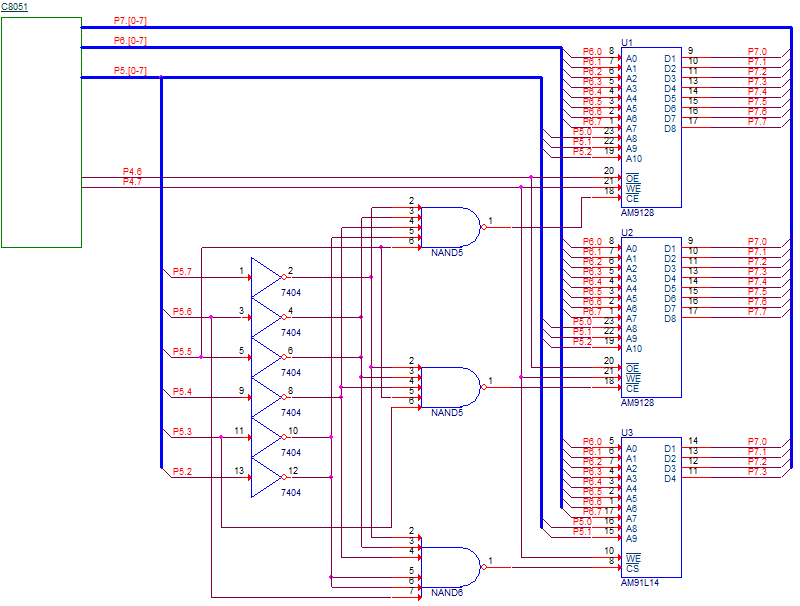
\includegraphics{schematic.png}
		\caption{Circuit schematic for parts 1 and 3}
		\label{schematic}
	\end{figure} 
\subsection{Part 1}
	\subsubsection{Code}
		\lstinputlisting{part1.c}
\subsection{Part 2}
	\subsubsection{Inaccurate timer code}
		\lstinputlisting{part2-1.c}
	\subsubsection{Accurate timer code}
		\lstinputlisting{part2-2.c}		

%\pagebreak
\subsection{Part 3}
	%\pagebreak
	\subsubsection{Code}
		\lstinputlisting{part3.c}
	
	
\section{References} 
\noindent
``MPS Lab 2," in RPI ECSE Department, 2016. [Online]. Available: \url{http://www.rpi.edu/dept/ecse/mps/MPS_Lab_Ex2-Intrpt.pdf}. Accessed: Sep. 22, 2016.\\
\newline\noindent
``C8051 Manual," in RPI ECSE Department, 1.4 ed., 2005. [Online]. Available: \url{https://www.ecse.rpi.edu/courses/CStudio/Silabs/C8051F12x-13x.pdf}. Accessed: Sep. 22, 2016.








\end{document}